% \cleardoublepage
\chapter{Approach and Design}\label{sec:approach_design}\minitoc\vspace{.5cm}
\index{Approach and Design}

By employing AF\_XDP sockets for the Receiver-Transmitter layer (RX-TX), we can achieve multipath tunneling that offers exceptional performance and grants complete control over raw IP packets before they enter the Linux network stack. 
Thanks to the secure design of the eBPF virtual machine architecture, this approach remains safer compared to utilizing kernel modules or kernel code used by Wireguard, OpenVPN, or IPsec.
In this chapter, we will explore the concept and design of the tunnel by examining its intended features and components.

\section{Multipath Tunnel using XDP socket}
% - A modern approach to system and network programming: performance, safe and free from legacy code thanks to eBPF technology.
% - Almost certainly will heavily outperform any other user-space approach
% - Increase redundancy and connection reliability.
% - Possible improvement in latency through efficiency and utilizing multipath.
% - Disparity in line utilization to support different types of streams: data need bandwidth, voice-over-ip needs low latency, critical message needs reliable transmission
At the conclusion of our project, we aim to provide an MTX library equipped with a comprehensive range of features, including:

\begin{itemize}
	\item Embrace a contemporary approach to system and network programming with the utilization of eBPF technology, ensuring performance, safety, and freedom from legacy code.
	\item Highly likely to outperform alternative user-space approaches significantly.
	\item Enhance redundancy and bolster connection reliability.
	\item Potential for improved latency by leveraging efficiency and harnessing the power of multipath.
	\item Address the varying requirements of different stream types by optimizing line utilization: bandwidth for data-intensive tasks, low latency for voice-over-IP, and reliable transmission for critical messages.
\end{itemize}

% - The MTX tunnel allows setting policies at several layers defined by algorithms or configuration. With such preemptive points these will be a large pool of configurations to chose from:
% 	- Data link layer: which stream can use which link, with which priority, what is the load distribution policy?
% 	- Network layer: select IPv4/v6 as carrier, which UDP port.
% 	- Application layer: priority of application, buffer fetching timeout, buffer reserved for low-latency usage, ...
% - Ideally, after initiation, a tunnel control plane will run in background and manage the streams that are used by several applications. These applications register usage to the tunnel control plane and interact with data plane through shared buffers. Parameters can be set individually for each app.
% - Apart from that, we will also investigate the possibility to create a TUN/TAP interface as a intermediate communicate layer between the MTX tunnel and apps. This is a well-known practice used by many VPN programs to allow several apps to use the VPN connection. This way, applications can use the tunnel connection without modifying the source code.
The MTX tunnel incorporates a flexible policy framework at multiple layers, enabling the utilization of algorithms or configurations. 
This offers a wide array of options for customization, including at:
\begin{itemize}
	\item Data link layer: determining which streams can utilize specific links, assigning priorities, and implementing load distribution policies.
	\item Network layer: selecting the carrier protocol (IPv4/v6) and specifying the UDP port.
	\item Application layer: prioritizing applications, defining buffer fetching timeouts, reserving buffers for low-latency usage, and more.
\end{itemize}

Ideally, a tunnel control plane will operate in the background after initiation, effectively managing the streams utilized by various applications. 
These applications will register their usage with the tunnel control plane and interact with the data plane through shared buffers. 
Parameters can be individually configured for each application.
Additionally, we will explore the feasibility of creating a TUN/TAP interface to serve as an intermediate communication layer between the MTX tunnel and applications. 
This approach, commonly employed by VPN programs, enables multiple applications to utilize the tunnel connection without requiring modifications to their source code.

\section{AF\_XDP socket - eBPF}
\subsection{Introduction to eBPF and Linux's kernel space}
% The kernel serves as the core program of an operating system. 
% In a computer system, multiple processes run simultaneously, each carrying out its designated tasks. 
% However, these processes are receptive and have limited access to information.
% A process cannot initiate or terminate other processes, including itself. 
% It is isolated and unable to communicate directly with other processes or devices.
% It lacks knowledge about its runtime, when it can run or has to stop or the specific memory location it occupies, whether in RAM or swap.
% Conversely, the kernel acts as the housekeeper, managing the hardware resources of the computer and allocating them to all processes. 
% It facilitates the execution of processes, schedules their runtime slots, and mediates communication and events between processes and hardware.
% Moreover, the kernel takes on responsibilities such as memory management, providing a file system, establishing networking capabilities, and offering the system's \ac{API} 
The kernel functions as the central program of an operating system, overseeing its core operations. 
In a computer system, numerous processes execute concurrently, each fulfilling its assigned tasks. 
However, these processes possess limited access to its surrounding information and are inherently passive.
For instance, a process lacks the ability to initiate or terminate other processes, including itself. 
It operates in a isolated virtual memory and lacks direct communication channels with other processes or devices. 
Furthermore, it lacks awareness of its runtime availability, including when it can execute or must cease, as well as knowledge of its specific memory location, whether in RAM or swap.
Conversely, the kernel assumes the role of a housekeeper, managing the hardware resources of the computer and allocating them among all processes. It facilitates process execution, schedules runtime slots, and mediates communication and events between processes and hardware components.
In addition to these responsibilities, the kernel handles vital tasks such as memory management, providing a file system, establishing networking capabilities, and presenting the system's \ac{API} for programmatic access \cite{kerrisk_linux_2010}.

% Linux's virtual memory is separated into kernel space and user space, which offers many advantages including increasing security and system's stability \cite{understanding_the_linux_kernel_bovet_cassetti}.
Linux's virtual memory architecture divides the memory into two distinct spaces: kernel space and user space. This separation provides several advantages, such as enhancing system security and stability \cite{understanding_the_linux_kernel_bovet_cassetti}.
% On Linux, a task can be processed in 2 modes: kernel mode and user mode.
% The CPU can't access memory that is marked as being used in kernel space when it is running in user mode 
In Linux, tasks can operate in two distinct modes: kernel mode and user mode. When running in user mode, the CPU is restricted from accessing memory allocated for kernel space \cite{kerrisk_linux_2010}.
Invisible to end user, the system switches between kernel mode and user mode very often, usually when a system \ac{API} is involved or a resource needs to be accessed \cite{Robert_linux_kernel_dev}.
% Although switching between modes is supported by the CPU, significant overhead is caused by switching context and translating memory address.
% Running code purely in the kernel space could reduce such overhead and have better scheduling policy, however this faces the risk of compromising the system through memory leak, crashing or malicious exploit 
Although the CPU supports mode switching, there is a noticeable overhead associated with context switching and memory address translation. 
Running code exclusively in the kernel space has the potential to reduce this overhead and enjoy \textit{better} scheduling policies. 
However, such an approach carries inherent risks, including the possibility of system compromise due to memory leaks, crashes, or malicious exploits \cite{lwn_detect_kernel_mem_leak} \cite{emamdoost_detecting_2021}.
% \ac{BPF} technology is a alternative tool to execute code in kernel space in a controlled environment.
% It was introduced in 1992 for \ac{BSD} OS and ported to Linux later. 
% Originated designed for network packet filtering, it has been since then extended and used for firewall, tracing, debugging purposes \cite{McCanne_intro_bpf} \cite{lwn_intro_ebpf} by tech giants: firewall, filter, load-balancer by Facebook \cite{facebook_katran_ebpf_2018}; monitoring and analyzing by Netflix \cite{netflix_network_insight}; security and observation by Cilium Project \cite{cilium_io_page}; cloud infrastructure by Alibaba \cite{alibaba_cloud_ebpf}.

\ac{BPF} technology provides an alternative means of executing code within the kernel space, offering a controlled environment for such operations. 
Initially introduced in 1992 for the \ac{BSD} OS, it was later ported to the Linux platform. 
Originally designed for network packet filtering, \ac{BPF} has since been expanded and utilized for purposes such as firewall management, tracing, and debugging \cite{McCanne_intro_bpf} \cite{lwn_intro_ebpf}. 
Prominent technology companies have leveraged \ac{BPF} for various applications, including: Facebook for firewall, filtering, and load balancing \cite{facebook_katran_ebpf_2018}; Netflix for network monitoring and analysis \cite{netflix_network_insight}; Cilium Project for security and observability purposes \cite{cilium_io_page} and Alibaba for their cloud infrastructure \cite{alibaba_cloud_ebpf}.

\begin{figure}[H]
    \centering
    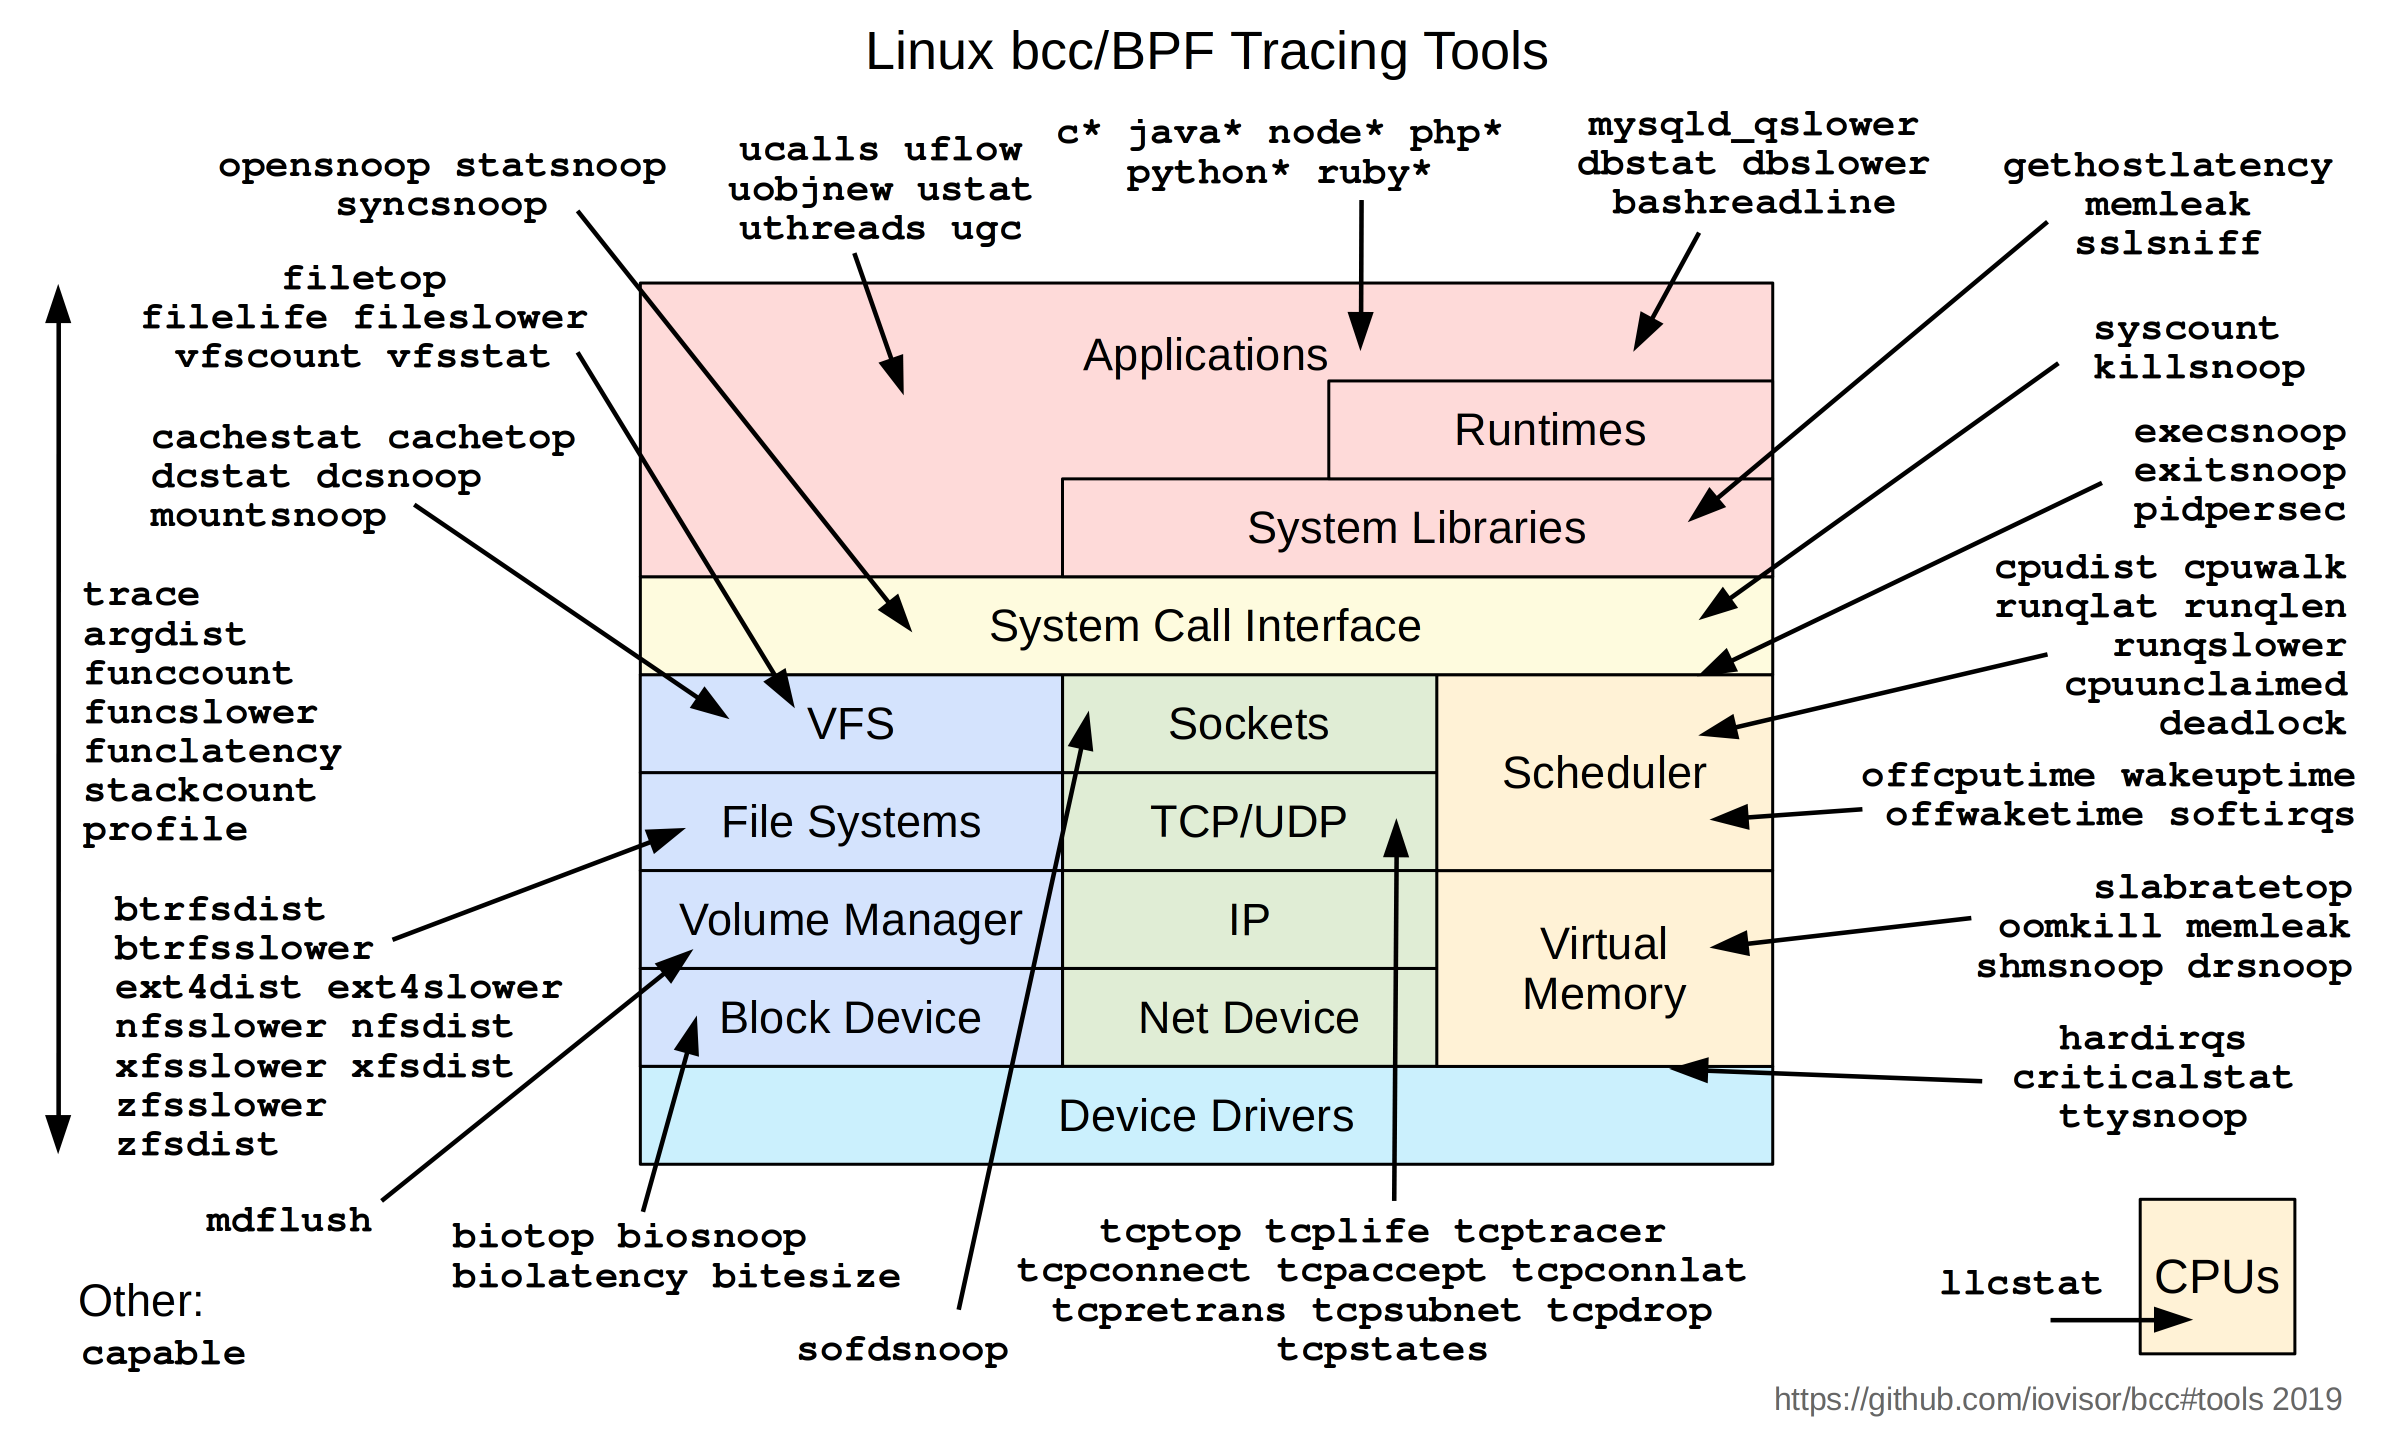
\includegraphics[width=1.0\textwidth]{resources/images/bcc_tracing_tools_2019.png}
    \caption{A wide range of Linux eBPF-based tracing tools \cite{iovisor_page}.}\label{fig:approach_design:tracing_tools_linux}
\end{figure}

\ac{ebpf} - the descendant of \ac{BPF} technology - consisted of a \ac{ebpf} program (also called \textit{kernel program}), the \ac{ebpf} virtual machine provided by the kernel, and the attach code path.
The \ac{ebpf} kernel program is written in a subset of the C programming language and compiled to \ac{ebpf} byte code.
The 64 bit \ac{RISC}-based \ac{ebpf} virtual machine along with a verifier check the code safety and isolate the execution of the \ac{ebpf} kernel program.
To get started, the kernel program is inserted to the desired code path in the kernel where it will be executed whenever the code path is traversed \cite{lwn_intro_ebpf}.

\subsection{AF\_XDP socket}

\begin{figure}[H]
	\centering
	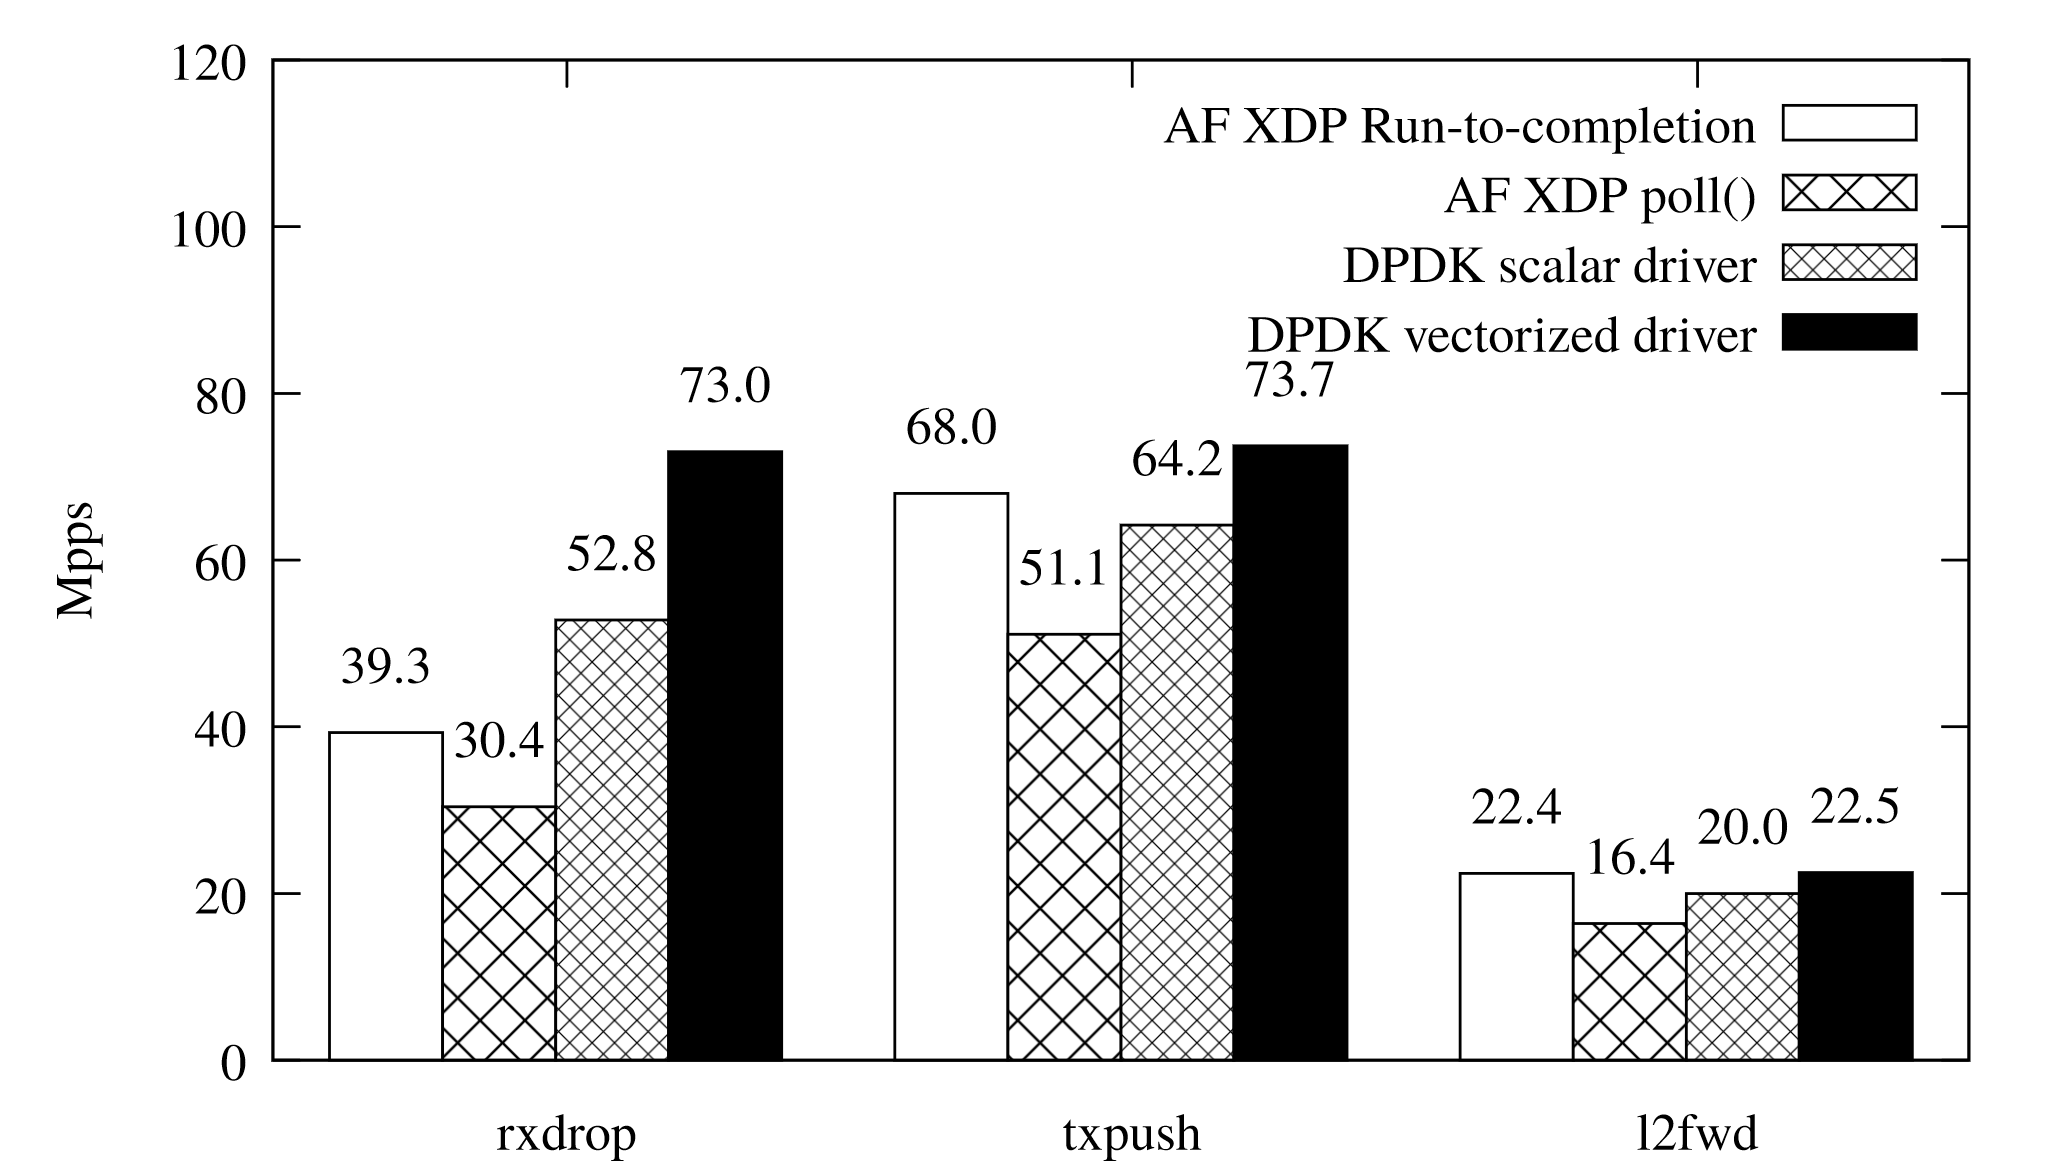
\includegraphics[width=0.8\textwidth]{af_xdp_vs_dpdk_3_micro_benchmarks.PNG}
	\caption{Comparing performance between \ac{xdppage} and \ac{dpdkpage} \cite{karlsson_path_to_dpdk_speednodate}. The authors tested  rxdrop (dropping all arriving packets), txpush (pushing packets out a NIC) and l2fwd (Level-2-forwarding, replacing MAC address of incoming packets and pushing them out) scenarios. DPDK continues to be the leading solution in terms of raw performance.}\label{fig:approach_design:af_xdp_vs_dpdk_3_micro_benchmarks}
\end{figure}

\ac{xdppage} is a type of Linux socket that utilizes \ac{ebpf} to deliver incoming raw network packets arrived from a \ac{NIC} to user space with comparable performance to \ac{dpdkpage} \cite{karlsson_path_to_dpdk_speednodate}. 
The socket has demonstrated the capability to fully utilize a 100Gb line per core on modern CPUs, with impressive baseline packet drop rates of up to 24 million packets per second (Mpps) compared to 4.8Mpps with Linux network stack \cite{hoiland_jorgensen_express_2018} \cite{intel_dpdk_perf}.
This high throughput potential allows us to establish multi-hundreds Gb connections (tunnels) by leveraging a few readily available 40/100Gb NICs, presenting a valuable opportunity for enhanced network performance.

Being a native Linux's feature, \ac{xdppage} has several advantages over other 3rd party solutions:
\begin{itemize}
	\item Reducing dependency: minimizing the reliance on third-party libraries reduces the concern for potential vulnerabilities.Furthermore, this approach guarantees the longevity of the product, as the socket is maintained by the dedicated team of kernel developers, indicating that the project is unlikely to be discontinued in the near future. 
	\item License: no special license required. However, the eBPF kernel program must be licensed under GNU \ac{GPL} since anything uses eBPF in kernel space is considered a derivative work \cite{gpl_email_discussion} \cite{linux_license_rule} \cite{lwn_clarify_bpf_license}.
	\item Security and Update: the open-source and collaborative nature of Linux ensures that its code base is diligently maintained by dedicated maintainers and an active community of contributors, including researcher from universities and institutes, employee from industrial vendors and individual hobbyist.
\end{itemize}

\begin{figure}[H]
	\centering
	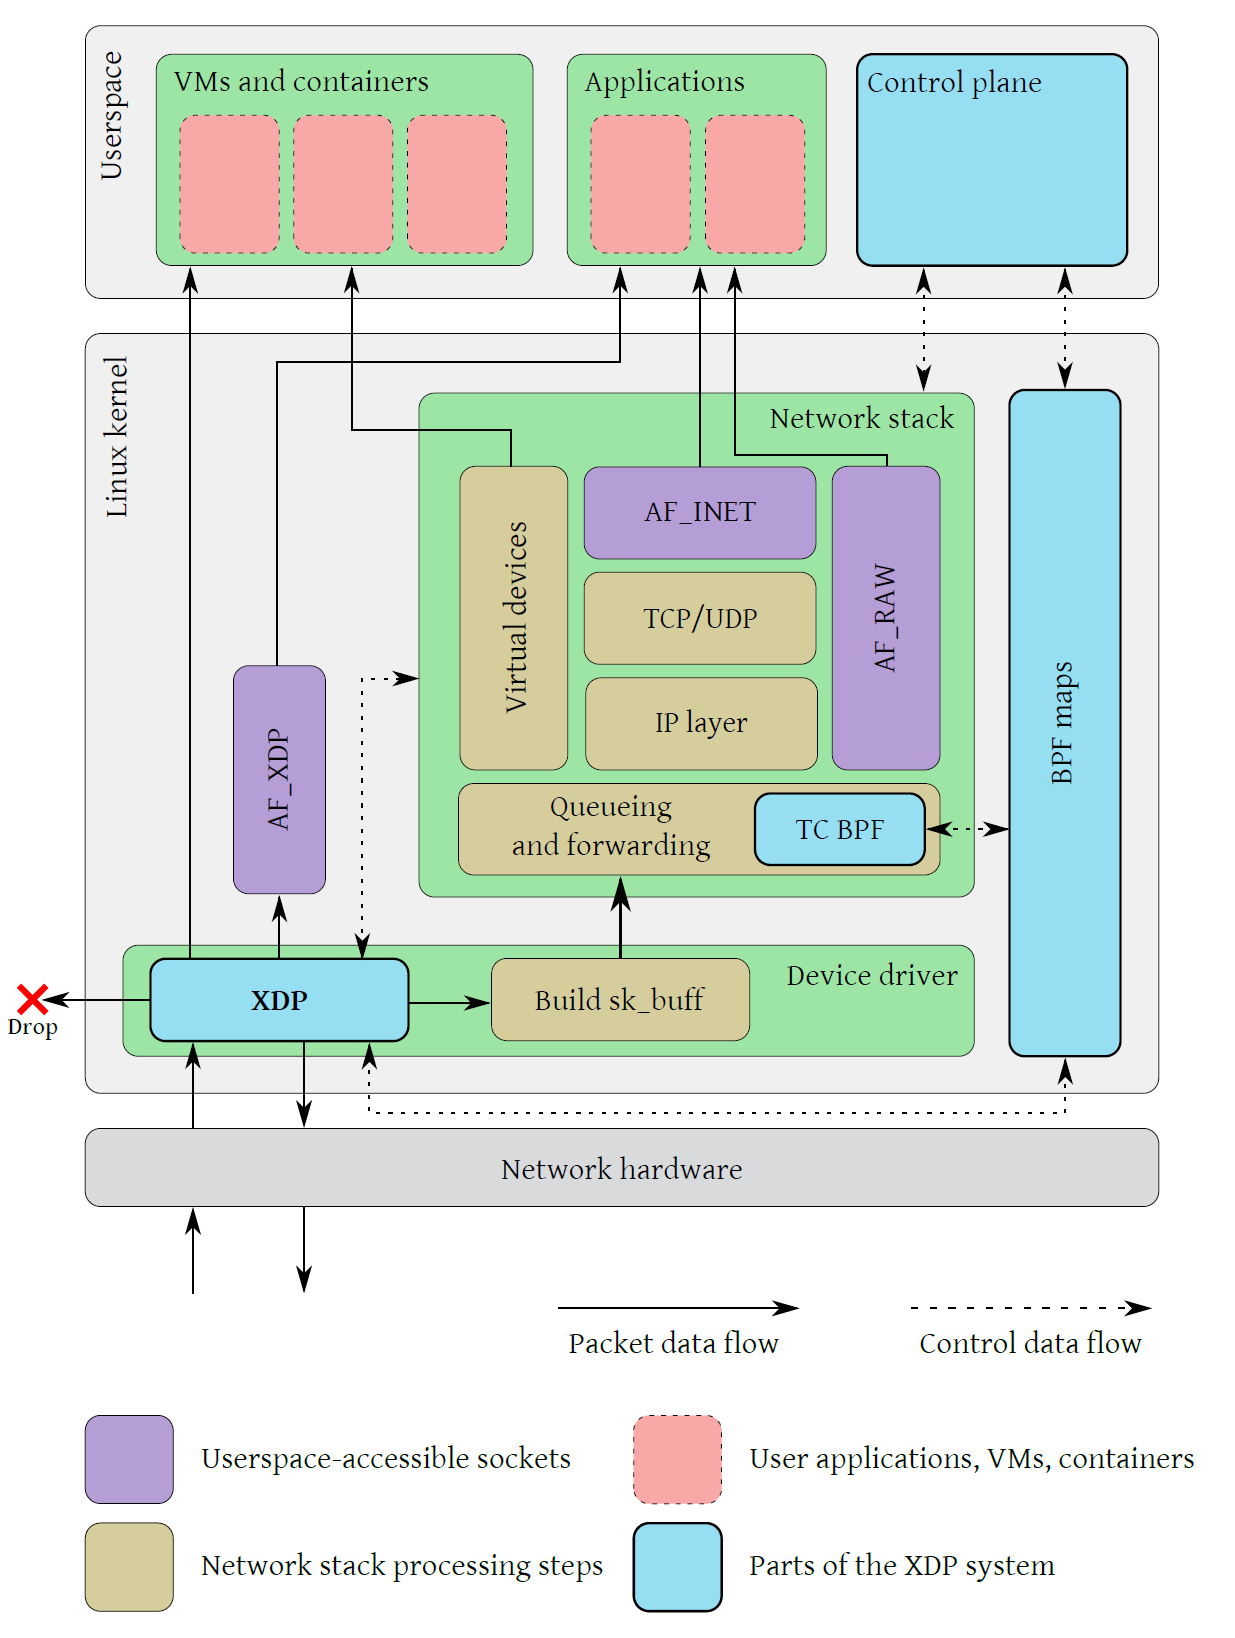
\includegraphics[width=1.0\textwidth]{XDP_integration_with_the_Linux_network_stack.PNG}
	\caption{XDP’s integration with the Linux network stack \cite{hoiland_jorgensen_express_2018}. The XDP program is activated whenever a packet enter the driver's buffer, where it will be examined. The XDP program makes the decision if the packet should follow its normal path in the network stack, or be discarded/forwarded/delivered to XDP user space program.}\label{fig:approach_design:xdp_architecture}
\end{figure}


\section{Implementation details}

\begin{figure}[H]
	\centering
	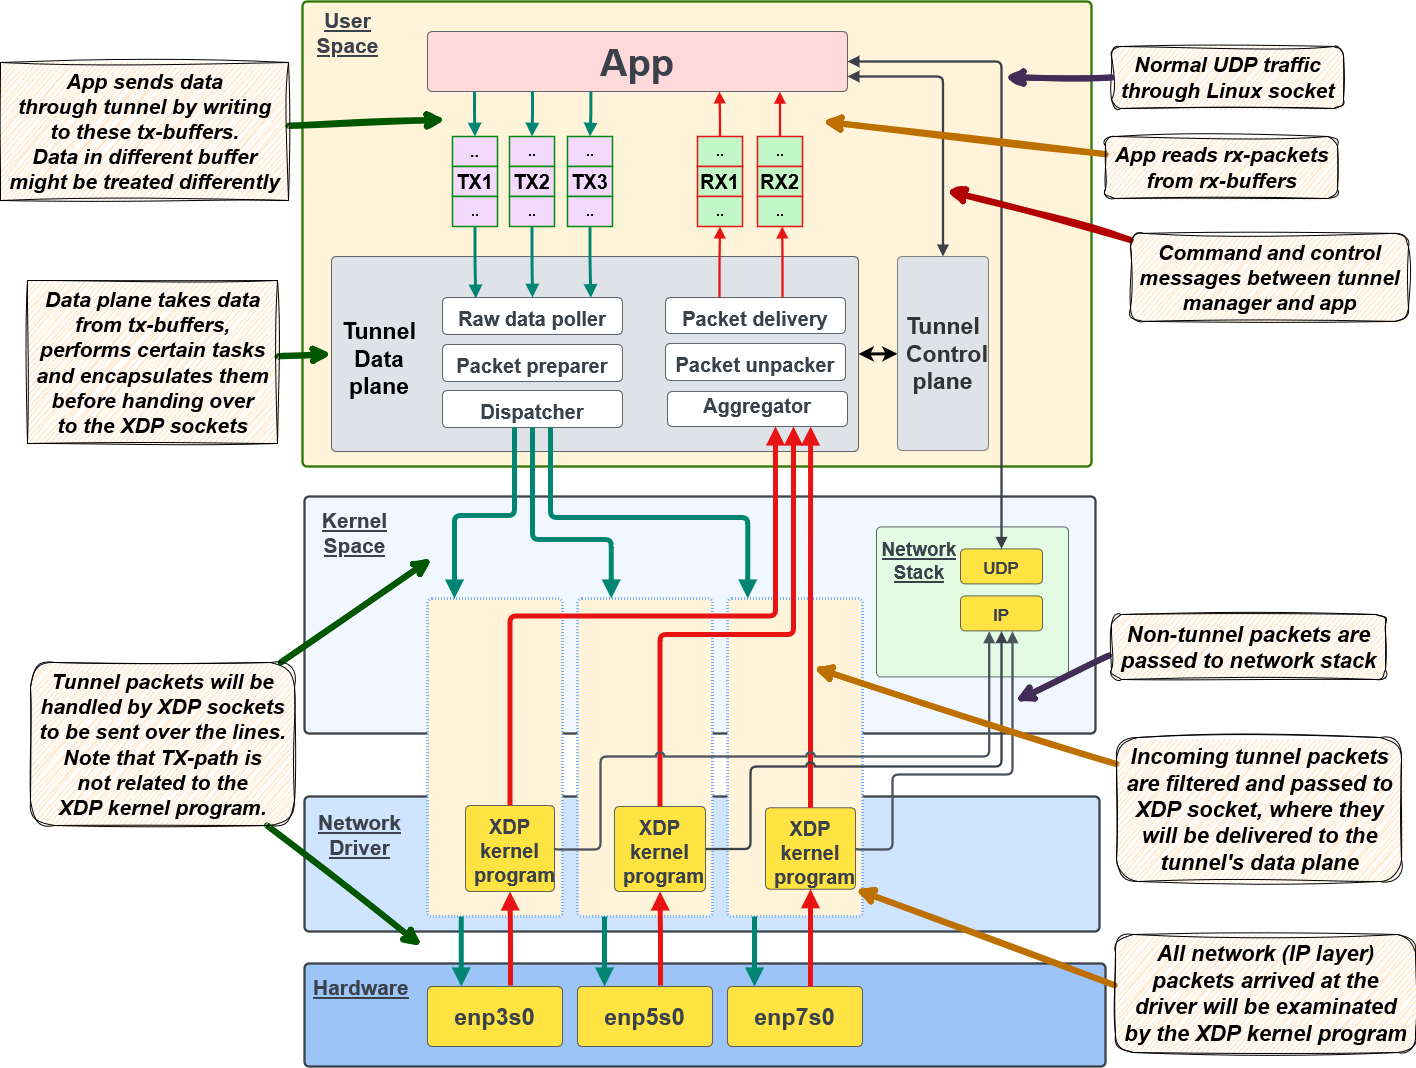
\includegraphics[width=1.0\textwidth]{mtx_design_and_workflow.png}
	\caption{The architecture of our MTX tunnel and the flow of packets. The notation \textit{1, 2 and 3} describe how  packets from application travel through the egress path. Notation \textit{4 to 8} show how application receive the packets from tunnel and normal Linux socket.}
	\label{fig:approach_design:mtx_design_and_workflow}
\end{figure}

The tunnel will be implemented in C for Linux. It consisted of 4 main components: eBPF kernel program, shared buffer, data plane and control plane.

\subsection{Buffers}
Buffers are separated into tx (transmit, see notation \textit{1}) and rx (receive, see notation \textit{8}) buffers that are available for application use. 
These buffers facilitate efficient data transfer for different streams and priorities, allowing the application to write to or read from the appropriate buffer as needed.

\subsection{Kernel Program}
XDP kernel program (see notation \textit{4}) is responsible for filtering tunnel packets based on criteria like UDP port, IP address, and the magic number in the tunnel header. 
These filtered packets are then delivered to the Packet aggregator for subsequent processing (notation \textit{5}). 
Conversely, all other packets that are not of interest to us are passed through to the Linux network stack (notation \textit{6 and 9}).
While it may be tempting to offload additional tasks such as unpacking and decryption to the kernel program for improved performance, it is important to note that this approach would significantly increase development time.

\subsection{Data Plane}
Data plane functionality is divided into two main paths: the TX path and the RX path.
\begin{itemize}
	\item TX path is responsible for data output and tunnel packet transmission. It consists of a poller that retrieves fresh packet data from the TX buffers, taking into account priorities for efficient processing. The poller determines the order in which packets are polled, considering factors such as smaller batch sizes and shorter timeouts to minimize waiting time and increase CPU usage. High-priority packets are processed first. After polling, the packet preparer handles tasks such as encryption, compression, and encapsulation. Finally, the dispatcher sends the prepared packets to the XDP sockets, which will then transmit them over the appropriate network links.
	\item RX path is responsible for receiving tunnel packets. The aggregator retrieves tunnel packets from the XDP sockets, and then passes them to the unpacker for unpacking and subsequent delivery to the RX buffers for further processing.
\end{itemize}

\subsection{Control Plane}
The control plane plays a vital role in the system as it handles various interactions with the application (notation \textit{7}). 
It is responsible for configuration management, initiation, termination, and runtime information exchange. 
The control plane acts as the central control hub, governing and coordinating all other components of the tunnel.

% \begin{itemize}
%     \item Top level
%     \begin{itemize}
%         \item Second level
%     \end{itemize}
% \end{itemize}
% \lstinputlisting{somefile}
% \begin{itemize}
%     \item[]\begin{itemize}
%         \item Second level
%     \end{itemize}
% \end{itemize}

% \section{Introduction}

% \begin{wrapfigure}{r}{0.2\textwidth}
%     \centering
%     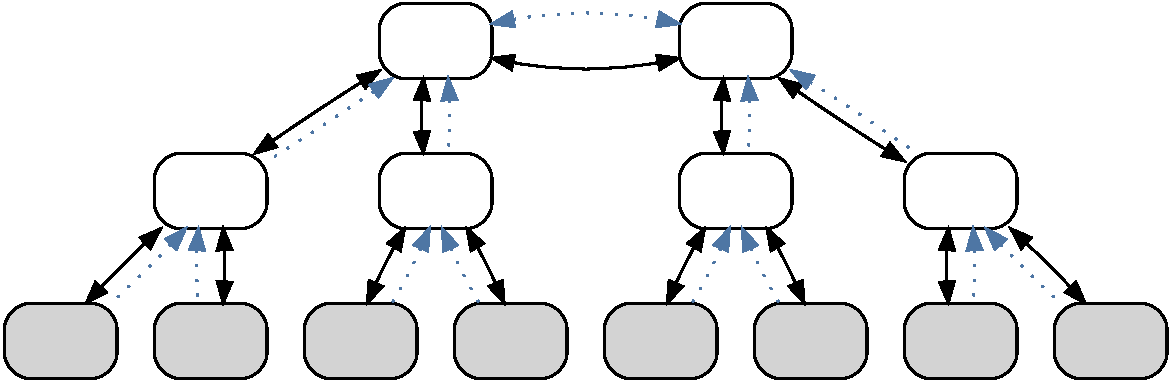
\includegraphics[width=0.2\textwidth]{resources/images/example3}
% \end{wrapfigure}

% \sidenote{Overview}
% \todomid{write about \Cref{fig:req:details}}

% \begin{figure}[H]
%     \centering
%     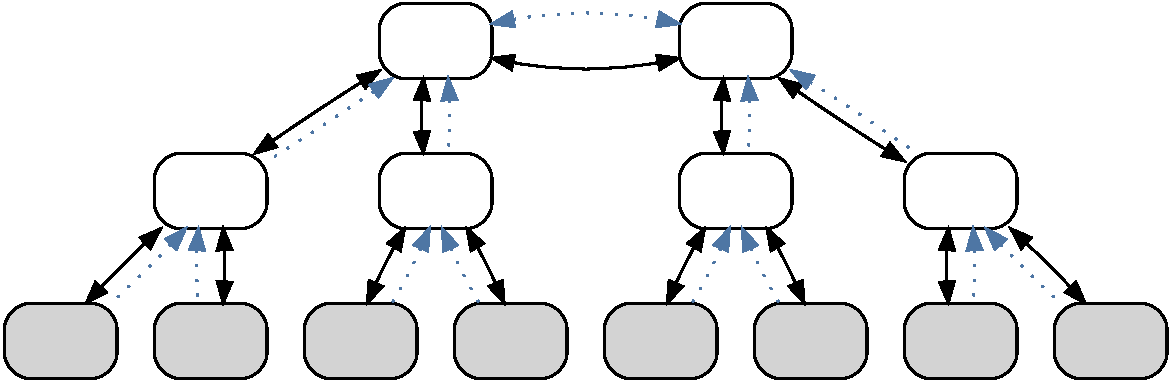
\includegraphics[width=.85\textwidth]{resources/images/example3}
%     \caption{More detailed overview of the requirements}\label{fig:req:details}
% \end{figure}

% \sidenote{Structure of Research}
% \todomid{write about \Cref{fig:hourglass:reqs}}

% \begin{figure}[H]
%     \centering
%     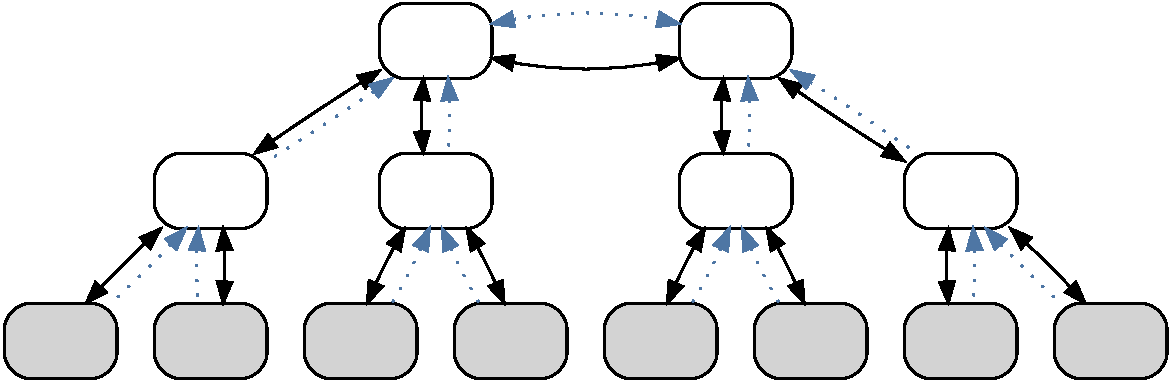
\includegraphics[width=.55\textwidth]{resources/images/example3}
%     \caption{Placement of the requirement section in the structure of research}\label{fig:hourglass:reqs}
% \end{figure}

% \section{Stakeholder 1}

% \sidenote{\Cref{tbl:reqs:stakeholder1}}
% \todomid{write about \Cref{tbl:reqs:stakeholder1}}

% \begin{tabularx}{\textwidth}{lX}
%     \caption{Requirements from stakeholder 1 perspective}\label{tbl:reqs:stakeholder1}\\
%     \toprule
%     \textbf{\#}& \textbf{Description}  \\\midrule
%     \endfirsthead%
%     \toprule
%     \textbf{\#}& \textbf{Description}  \\\midrule
%     \endhead%
%     \requirement{U}{req:stakeholder1:foo}{Foo}
%        & \todomid{write}
%     \\\midrule
%     \requirement{U}{req:stakeholder1:bar}{Bar}
%        & \todomid{write}
%     \\\bottomrule
% \end{tabularx}

% \section{Stakeholder 2}

% \sidenote{\Cref{tbl:reqs:stakeholder2}}
% \todomid{write about \Cref{tbl:reqs:stakeholder2}}

% \begin{tabularx}{\textwidth}{lX}
%     \caption{Requirements from stakeholder 2 perspective}\label{tbl:reqs:stakeholder2}\\
%     \toprule
%     \textbf{\#}& \textbf{Description}  \\\midrule
%     \endfirsthead%
%     \toprule
%     \textbf{\#}& \textbf{Description}  \\\midrule
%     \endhead%
%     \requirement{S}{req:stakeholder2:foo}{Foo}
%        & \todomid{write}
%     \\\midrule
%     \requirement{S}{req:stakeholder2:bar}{Bar}
%        & \todomid{write}
%     \\\bottomrule
% \end{tabularx}

% \section{Stakeholder 3}

% \sidenote{\Cref{tbl:reqs:stakeholder3}}
% \todomid{write about \Cref{tbl:reqs:stakeholder3}}

% \begin{tabularx}{\textwidth}{lX}
%     \caption{Requirements from stakeholder 3 perspective}\label{tbl:reqs:stakeholder3}\\
%     \toprule
%     \textbf{\#}& \textbf{Description}  \\\midrule
%     \endfirsthead%
%     \toprule
%     \textbf{\#}& \textbf{Description}  \\\midrule
%     \endhead%
%     \requirement{T}{req:stakeholder3:foo}{Foo}
%        & \todomid{write}
%     \\\midrule
%     \requirement{T}{req:stakeholder3:bar}{Bar}
%        & \todomid{write}
%     \\\bottomrule
% \end{tabularx}

% \section{Conclusion}

% \sidenote{Summary}
% \todomid{write}

% \sidenote{Takeaway 1}
% \todomid{write}

% \sidenote{Takeaway 2}
% \todomid{write}

% \sidenote{Takeaway 3}
% \todomid{write}

% \sidenote{Next chapter}
% \todomid{write}
